\section{Methods}
\label{method}

\subsection{Datasets and workflow}

The repository contains a table-driven registry of 26 ENCODE eCLIP datasets
covering 15 RBPs in K562 and HepG2 cells. Each entry specifies two deduplicated
IP BAM files, an SMInput BAM file, a GRCh38 reference, benchmark regions, and
RBP-specific motif information. The experiments analyzed in this report use
PUM2, HNRNPK, U2AF2, QKI, and PUM1 in K562 cells. PureCLIP was restricted to
chromosome~21 to make iterative evaluation tractable. Reference regions were
restricted to the same chromosome before recall was calculated.

Both optimizers call the same \texttt{evaluate\_config()} entry point
(Figure~\ref{fig:pipeline}). The Snakemake workflow merges the IP replicates,
runs PureCLIP on the merged BAM and separately on each replicate, converts raw
calls into standardized footprints, and calculates the evaluation metrics. Each
trial writes its parameters and scores to a self-contained
\texttt{score\_report.json} file.

\begin{figure}[H]
\centering
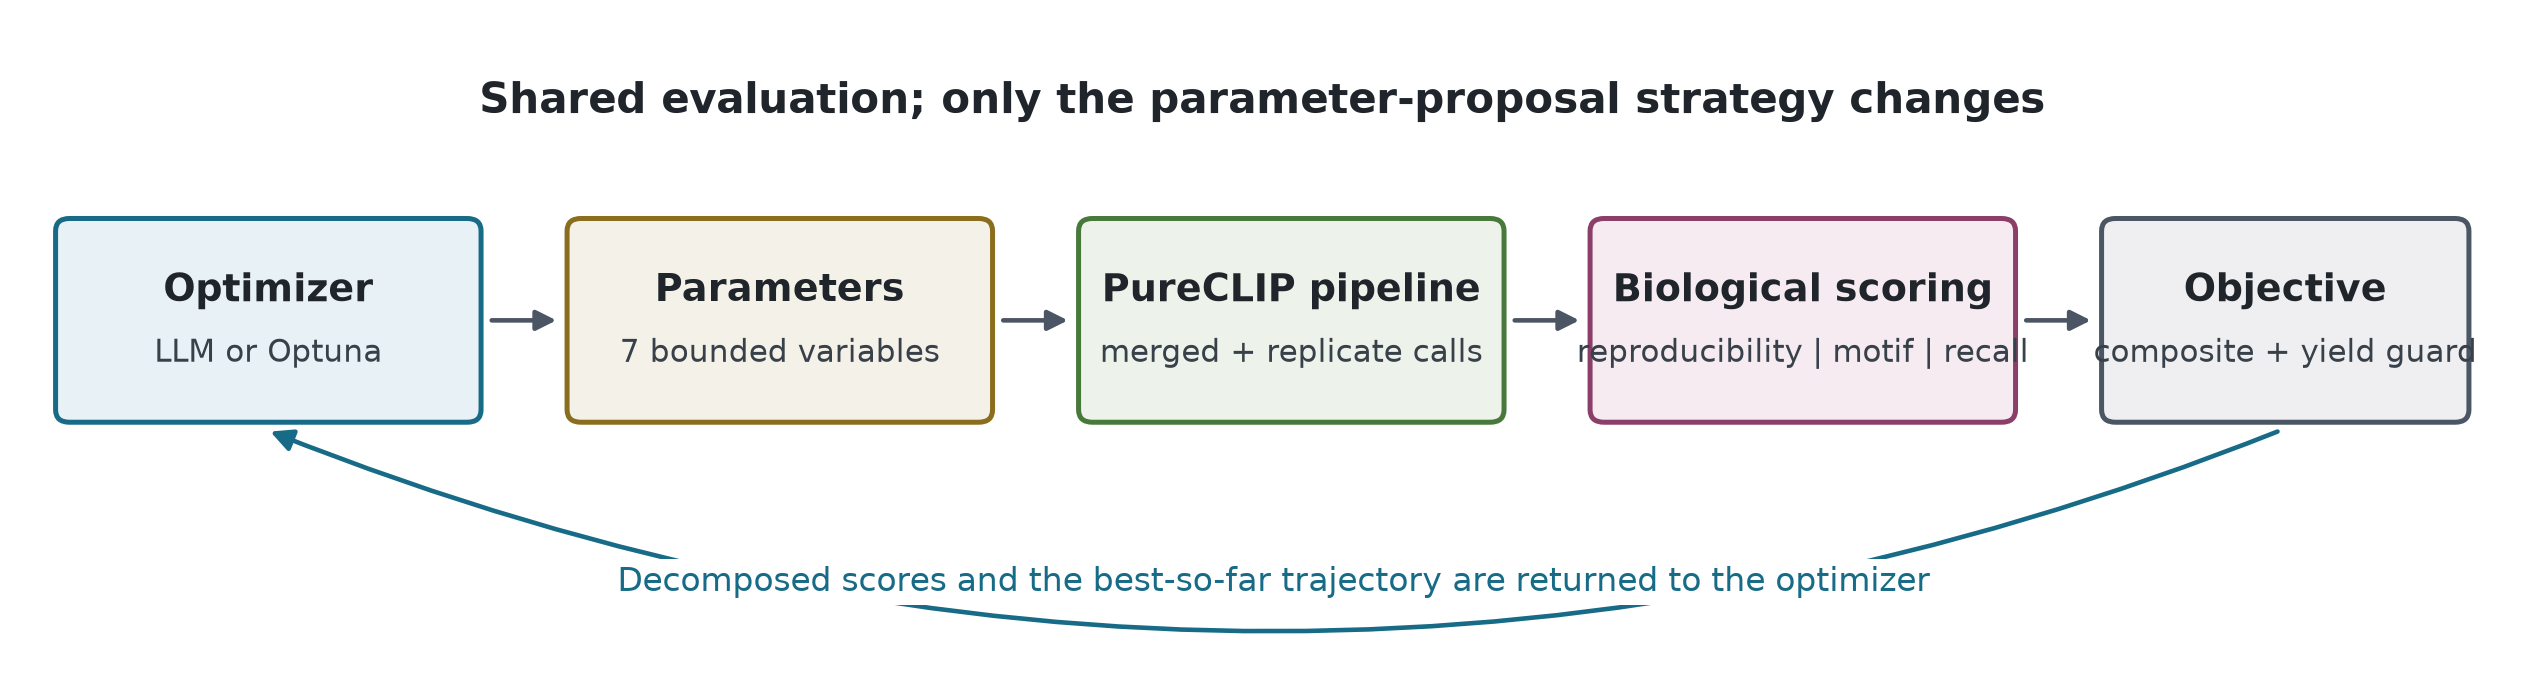
\includegraphics[width=\linewidth]{images/pipeline_overview.png}
\caption{Shared optimization workflow. The LLM and TPE differ only in how they
propose parameters. All candidates are evaluated by the same PureCLIP,
post-processing, and scoring implementation.}
\label{fig:pipeline}
\end{figure}

\subsection{Search space}

Seven integer or binary variables were optimized (Table~\ref{tab:params}). The
bounds were fixed for every arm. Four variables control PureCLIP and three
control the conversion of raw crosslink calls into binding-site footprints.

\begin{table}[H]
\centering
\small
\begin{tabular}{@{}llll@{}}
\toprule
Stage & Parameter & Range & Function \\
\midrule
PureCLIP & \texttt{bandwidth\_nt}          & 20--100 & signal smoothing \\
         & \texttt{merge\_distance\_nt}    & 4--16   & merge nearby events \\
         & \texttt{high\_precision\_mode} & \{0,1\} & change calling stringency \\
         & \texttt{use\_input\_covariate} & \{0,1\} & include SMInput signal \\
Post-processing & \texttt{min\_crosslink\_events} & 2--6 & filter weak sites \\
                & \texttt{force\_width}          & 3--15 & standardize site width \\
                & \texttt{cluster\_gap\_width}   & 4--16 & cluster adjacent calls \\
\bottomrule
\end{tabular}
\caption{Parameter space used by both optimization strategies.}
\label{tab:params}
\end{table}

\subsection{Composite objective}

For a call set with $n$ sites, the objective was
\begin{equation}
S = \left(0.50R_\mathrm{rep}+0.25R_\mathrm{motif}+0.25R_\mathrm{ref}\right)
\min\!\left(1,\frac{n}{10}\right),
\label{eq:composite}
\end{equation}
where $R_\mathrm{rep}$ is chance-corrected replicate agreement,
$R_\mathrm{motif}$ is the selected PWM hit rate, and $R_\mathrm{ref}$ is recall
of chromosome-21 reference regions. All terms are bounded by zero and one. The
final factor penalizes call sets with fewer than ten sites. This guard was
introduced after preliminary searches produced small call sets with high
agreement and motif fractions but negligible genomic coverage. When a component
is unavailable, the implementation renormalizes the weights over the remaining
components; all records used in the reported comparison contained all three.

\subsection{Experimental conditions}

The principal experiment contains three arms for PUM2, HNRNPK, and U2AF2. The
\emph{LLM-with-prior} arm used DeepSeek \texttt{deepseek-chat} at low temperature
\parencite{deepseek2024} and received the RBP identity, known motifs, an expected
footprint, the parameter
bounds, the current configuration, and the decomposed score trajectory. The
\emph{LLM-without-prior} arm received the same bounds, metrics, and trajectory,
but not the RBP identity or biological context. Thus, the ablation isolates the
information supplied in the biological prior; it does not remove numerical
feedback. Proposed JSON changes were validated against the search bounds and
retried after invalid responses. The \emph{TPE} arm used Optuna with seed 42 and
observed the scalar composite score.

All arms had a nominal cap of 16 evaluations and a stagnation threshold of 0.01
for four successive evaluations. For the LLM, counting began immediately. For
TPE, it began after the ten startup trials used by the sampler. Consequently,
the rule did not produce equal evaluation counts: completed LLM runs used five
to nine evaluations, whereas completed TPE runs used 14 to 16. The U2AF2 TPE run
was terminated by the batch time limit after two evaluations. QKI and PUM1 were
earlier pilot experiments under the same objective; the PUM1 TPE run also ended
at the batch time limit. All analyses are descriptive because each arm was run
once and no estimate of between-run variability is available.
